\documentclass[a4paper,12pt]{article}
\usepackage[utf8]{inputenc}
\usepackage[T1]{fontenc}
\usepackage[french]{babel}
\usepackage{graphicx}
\usepackage{hyperref}
\usepackage{listings}
\usepackage{xcolor}
\usepackage{geometry}
\usepackage{caption}
\usepackage{amsmath}
\usepackage{amssymb}

\geometry{margin=2.5cm}

% Configuration pour les listings de code
\definecolor{codebg}{RGB}{245,245,245}
\lstset{
    language=SQL,
    backgroundcolor=\color{codebg},
    basicstyle=\ttfamily\small,
    frame=single,
    breaklines=true,
    columns=fullflexible,
    keywordstyle=\color{blue},
    commentstyle=\color{gray},
    stringstyle=\color{orange},
    showstringspaces=false
}

\begin{document}

% Page de titre
\begin{titlepage}
    \centering
    \vspace*{5cm}
    {\Huge\bfseries Projet de Système de Base de Données pour le Site de Préférences Vidéo\par}
    \vspace{1cm}
    {\Large Rapport de Projet\par}
    \vspace{2cm}
    {\large \today\par}
    \vfill
\end{titlepage}

\tableofcontents
\newpage

\section{Aperçu du Projet}

Le but de ce projet est de concevoir et d'implémenter un système de base de données robuste pour un site de replay vidéo qui gère les inscriptions des utilisateurs, les détails des vidéos, l'historique de visionnage et les suggestions personnalisées de vidéos. La plateforme permettra aux utilisateurs d'explorer des vidéos par catégories, de suivre leurs favoris et de recevoir des recommandations personnalisées basées sur la popularité des vidéos. La base de données gérera également le cycle de vie des vidéos, y compris l'archivage du contenu plus ancien.

\section{Objectifs}

\begin{enumerate}
    \item \textbf{Développer une base de données relationnelle pour gérer :}
    \begin{itemize}
        \item \textbf{Informations des utilisateurs} : inscription, identifiants de connexion, détails du profil et préférences.
        \item \textbf{Détails des vidéos} : métadonnées, disponibilité, catégorisation et cycle de vie.
        \item \textbf{Activité des utilisateurs} : historique de visionnage, favoris et abonnements.
        \item \textbf{Suggestions} : recommandations personnalisées basées sur la popularité récente des vidéos.
    \end{itemize}
    \item \textbf{Assurer que la base de données peut supporter des fonctionnalités telles que :}
    \begin{itemize}
        \item Suivi de la disponibilité des vidéos et automatisation de l'archivage après l'expiration de la période de visionnage.
        \item Génération de suggestions de visionnage dynamiques pour les utilisateurs inscrits.
        \item Enregistrement des interactions des utilisateurs pour des expériences personnalisées et des analyses historiques.
    \end{itemize}
\end{enumerate}

\section{Portée}

\subsection{Entités de la Base de Données}

\subsubsection{Utilisateurs}

\textbf{Attributs} :
\begin{itemize}
    \item Identifiant (login)
    \item Mot de passe
    \item Nom de famille
    \item Prénom
    \item Date de naissance
    \item Email
    \item Préférences (catégories d'intérêt)
    \item Statut d'abonnement à la newsletter
\end{itemize}

\textbf{Fonctionnalités} :
\begin{itemize}
    \item Suivre les vidéos favorites.
    \item S'abonner à des émissions pour des suggestions automatiques.
    \item Accéder à l'historique de visionnage.
\end{itemize}

\subsubsection{Vidéos}

\textbf{Attributs} :
\begin{itemize}
    \item Nom
    \item Description
    \item Durée
    \item Date de sortie
    \item Pays d'origine
    \item Support multilingue
    \item Format d'image
    \item Statut de disponibilité (actif/archivé)
\end{itemize}

\textbf{Fonctionnalités} :
\begin{itemize}
    \item Catégorisées en genres (ex. : culture, cinéma).
    \item Support des émissions à plusieurs épisodes.
    \item Gestion du cycle de vie (disponibilité minimale de 7 jours, règles d'archivage).
\end{itemize}

\subsubsection{Historique de Visionnage}

\textbf{Attributs} :
\begin{itemize}
    \item ID utilisateur
    \item ID vidéo
    \item Date de visionnage
\end{itemize}

\textbf{Fonctionnalités} :
\begin{itemize}
    \item Maintenir un enregistrement des vidéos visionnées pour chaque utilisateur.
\end{itemize}

\subsubsection{Suggestions}

\textbf{Générées en fonction de} :
\begin{itemize}
    \item Popularité au sein des catégories (nombre de vues au cours des deux dernières semaines).
    \item Abonnements de l'utilisateur aux émissions.
\end{itemize}

\subsection{Principales Fonctionnalités}

\begin{enumerate}
    \item \textbf{Gestion des utilisateurs} :
    \begin{itemize}
        \item Permettre aux utilisateurs de créer des comptes, de se connecter et de gérer leurs préférences.
        \item Fournir l'option de s'abonner aux newsletters et à des catégories de programmes spécifiques.
    \end{itemize}
    \item \textbf{Cycle de vie des vidéos} :
    \begin{itemize}
        \item Archiver automatiquement les vidéos après une durée spécifique tout en assurant au moins 7 jours de disponibilité.
    \end{itemize}
    \item \textbf{Expérience de visionnage} :
    \begin{itemize}
        \item Permettre aux utilisateurs de marquer des vidéos comme favorites et de les afficher sur une page personnalisée.
        \item Mettre en évidence les vidéos proches de la fin de leur disponibilité.
    \end{itemize}
    \item \textbf{Système de recommandation} :
    \begin{itemize}
        \item Générer des suggestions basées sur la popularité des catégories au cours des deux dernières semaines.
    \end{itemize}
    \item \textbf{Analyse des données} :
    \begin{itemize}
        \item Suivre les vues des vidéos et les tendances de popularité.
    \end{itemize}
\end{enumerate}

\section{Entités}

Voici un aperçu détaillé des entités et de leurs attributs associés :

\subsection{Utilisateur}

\textbf{Attributs} :
\begin{itemize}
    \item \textbf{Login} (Identifiant unique)
    \item \textbf{Mot de passe}
    \item \textbf{Prénom}
    \item \textbf{Nom de famille}
    \item \textbf{Date de naissance}
    \item \textbf{Adresse email}
    \item \textbf{Catégories d'intérêt}
    \item \textbf{Abonnement à la newsletter hebdomadaire} (Booléen : Oui/Non)
\end{itemize}

\textbf{Relations} :
\begin{itemize}
    \item S'abonne à des émissions (Plusieurs-à-plusieurs avec \textit{Programme})
    \item Marque des vidéos comme favorites (Plusieurs-à-plusieurs avec \textit{Vidéo})
    \item A un historique de visionnage (Un-à-plusieurs avec \textit{Visionnage Vidéo})
\end{itemize}

\subsection{Vidéo}

\textbf{Attributs} :
\begin{itemize}
    \item \textbf{ID Vidéo} (Identifiant unique)
    \item \textbf{Nom}
    \item \textbf{Description}
    \item \textbf{Durée}
    \item \textbf{Date de sortie}
    \item \textbf{Pays d'origine}
    \item \textbf{Disponibilité multilingue} (Booléen : Oui/Non)
    \item \textbf{Format d'image}
    \item \textbf{Statut} (Disponible/Archivé)
\end{itemize}

\textbf{Relations} :
\begin{itemize}
    \item Appartient à un programme (Plusieurs-à-un avec \textit{Programme})
    \item Apparaît dans les favoris de l'utilisateur (Plusieurs-à-plusieurs avec \textit{Utilisateur})
    \item Vue dans l'historique de l'utilisateur (Un-à-plusieurs avec \textit{Visionnage Vidéo})
\end{itemize}

\subsection{Programme}

\textbf{Attributs} :
\begin{itemize}
    \item \textbf{ID Programme} (Identifiant unique)
    \item \textbf{Nom}
    \item \textbf{Catégorie} (ex. : Culture, Cinéma)
\end{itemize}

\textbf{Relations} :
\begin{itemize}
    \item Inclut des épisodes/vidéos (Un-à-plusieurs avec \textit{Vidéo})
\end{itemize}

\subsection{Visionnage Vidéo}

\textbf{Attributs} :
\begin{itemize}
    \item \textbf{ID Visionnage} (Identifiant unique)
    \item \textbf{ID Utilisateur} (Clé étrangère vers \textit{Utilisateur})
    \item \textbf{ID Vidéo} (Clé étrangère vers \textit{Vidéo})
    \item \textbf{Horodatage du visionnage}
\end{itemize}

\textbf{Relations} :
\begin{itemize}
    \item Suit l'historique de visionnage des vidéos de l'utilisateur (Plusieurs-à-un avec \textit{Utilisateur})
    \item Suit quelle vidéo a été visionnée (Plusieurs-à-un avec \textit{Vidéo})
\end{itemize}

\subsection{Catégorie}

\textbf{Attributs} :
\begin{itemize}
    \item \textbf{ID Catégorie} (Identifiant unique)
    \item \textbf{Nom}
\end{itemize}

\textbf{Relations} :
\begin{itemize}
    \item Associée à des programmes (Un-à-plusieurs avec \textit{Programme})
\end{itemize}

\subsection{Suggestions de Visionnage}

\textbf{Attributs} :
\begin{itemize}
    \item \textbf{ID Suggestion} (Identifiant unique)
    \item \textbf{Horodatage de génération}
    \item \textbf{Données de popularité de catégorie} (Nombre de vues au cours des deux dernières semaines)
\end{itemize}

\textbf{Relations} :
\begin{itemize}
    \item Vidéos suggérées (Un-à-plusieurs avec \textit{Vidéo})
\end{itemize}

\section{Création de la Base de Données}

J'ai utilisé \textbf{PostgreSQL 17} pour la gestion de la base de données.

\subsection{Scripts SQL de Création des Tables}

\begin{lstlisting}
-- 1. Table Utilisateurs
CREATE TABLE users (
    user_id SERIAL PRIMARY KEY,
    login VARCHAR(50) UNIQUE NOT NULL,
    password VARCHAR(255) NOT NULL,
    first_name VARCHAR(50),
    last_name VARCHAR(50),
    date_of_birth DATE,
    email VARCHAR(100) UNIQUE,
    interested_categories TEXT[], -- Tableau de categories
    newsletter_subscription BOOLEAN DEFAULT FALSE
);

-- 2. Table Categories
CREATE TABLE categories (
    category_id SERIAL PRIMARY KEY,
    name VARCHAR(50) UNIQUE NOT NULL
);

-- 3. Table Programmes
CREATE TABLE programs (
    program_id SERIAL PRIMARY KEY,
    name VARCHAR(100) NOT NULL,
    category_id INT REFERENCES categories(category_id) ON DELETE SET NULL
);

-- 4. Table Videos
CREATE TABLE videos (
    video_id SERIAL PRIMARY KEY,
    name VARCHAR(100) NOT NULL,
    description TEXT,
    duration INTERVAL NOT NULL,
    release_date DATE NOT NULL,
    country_of_origin VARCHAR(50),
    multi_language_available BOOLEAN DEFAULT FALSE,
    image_format VARCHAR(50),
    status VARCHAR(10) DEFAULT 'Available', -- 'Available' ou 'Archived'
    program_id INT REFERENCES programs(program_id) ON DELETE CASCADE
);

-- 5. Table Videos Favorites (Relation Plusieurs-a-plusieurs entre Utilisateurs et Videos)
CREATE TABLE favorite_videos (
    user_id INT REFERENCES users(user_id) ON DELETE CASCADE,
    video_id INT REFERENCES videos(video_id) ON DELETE CASCADE,
    PRIMARY KEY (user_id, video_id)
);

-- 6. Table Visionnage Video
CREATE TABLE video_viewings (
    viewing_id SERIAL PRIMARY KEY,
    user_id INT REFERENCES users(user_id) ON DELETE CASCADE,
    video_id INT REFERENCES videos(video_id) ON DELETE CASCADE,
    viewing_timestamp TIMESTAMP DEFAULT CURRENT_TIMESTAMP
);

-- 7. Table Suggestions de Visionnage
CREATE TABLE viewing_suggestions (
    suggestion_id SERIAL PRIMARY KEY,
    generated_timestamp TIMESTAMP DEFAULT CURRENT_TIMESTAMP,
    category_id INT REFERENCES categories(category_id) ON DELETE CASCADE,
    video_id INT REFERENCES videos(video_id) ON DELETE CASCADE
);

-- 8. Table Programmes Abonnes (Relation Plusieurs-a-plusieurs entre Utilisateurs et Programmes)
CREATE TABLE subscribed_programs (
    user_id INT REFERENCES users(user_id) ON DELETE CASCADE,
    program_id INT REFERENCES programs(program_id) ON DELETE CASCADE,
    PRIMARY KEY (user_id, program_id)
);
\end{lstlisting}

\subsection{Liste des Tables}

Après avoir exécuté les scripts, la requête suivante permet d'afficher la liste des tables :

\begin{lstlisting}
SELECT * FROM pg_catalog.pg_tables WHERE schemaname='public';
\end{lstlisting}

\begin{figure}[h!]
    \centering
    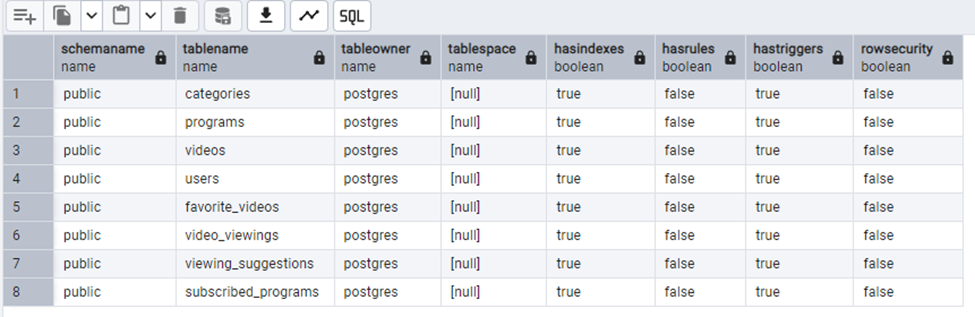
\includegraphics[width=0.8\textwidth]{photo1.jpg}
    \caption{Liste des tables}
\end{figure}

\section{Modèle Entité/Association}

\begin{figure}[h!]
    \centering
    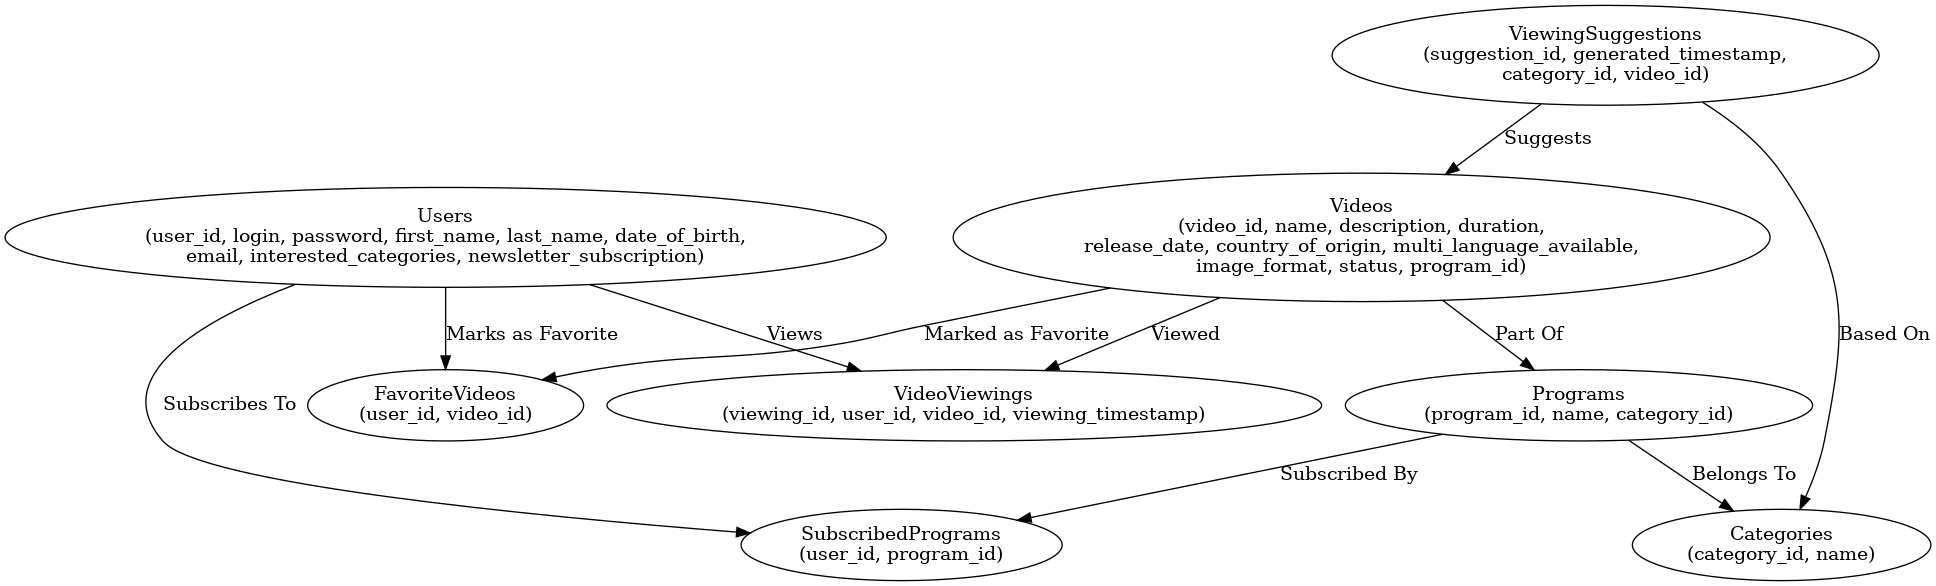
\includegraphics[width=0.9\textwidth]{photo2.jpg}
    \caption{Modèle E/A}
\end{figure}

Le modèle ERD est présenté ci-dessous :

\begin{figure}[h!]
    \centering
    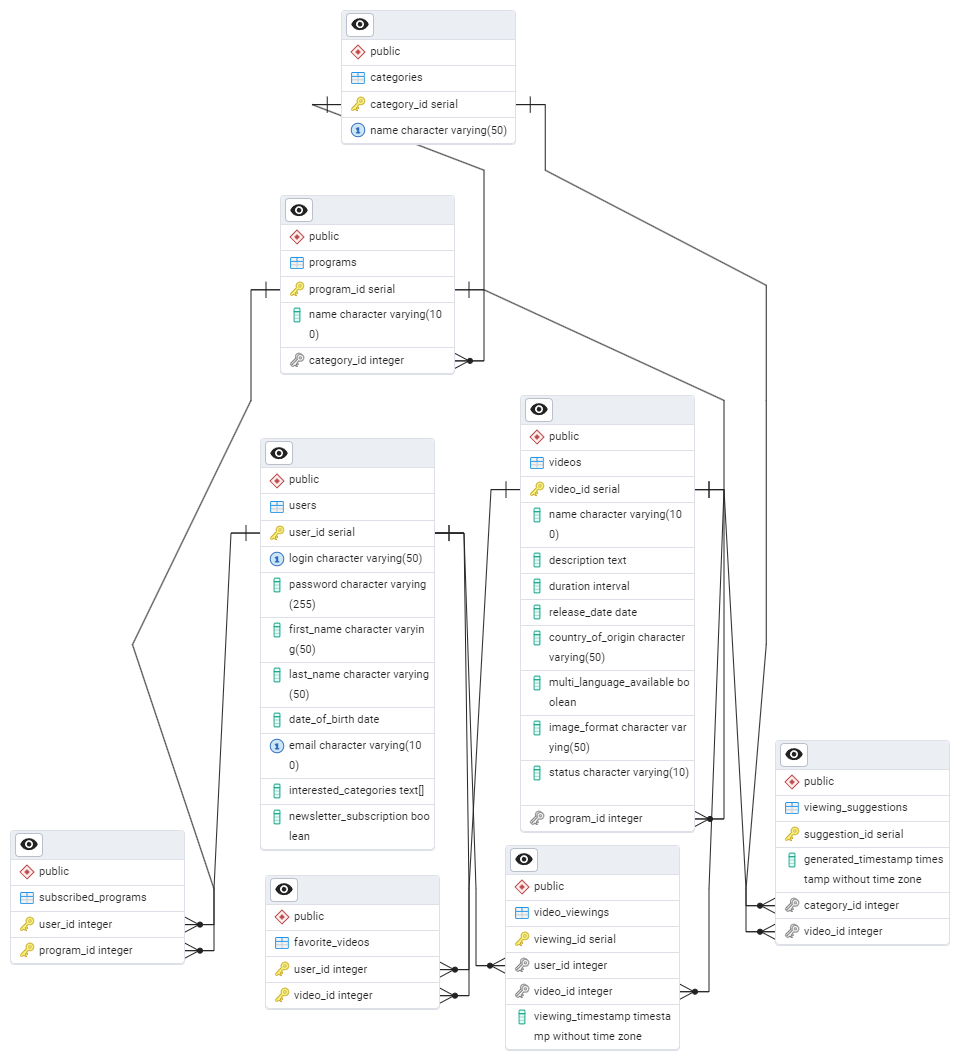
\includegraphics[width=0.9\textwidth]{photo3.jpg}
    \caption{Modèle ERD}
\end{figure}

\section{Requêtes SQL}

\subsection{Nombre de vues des vidéos par catégorie pour les vues datant de moins de deux semaines}

\begin{lstlisting}
SELECT 
    c.name AS category_name,
    COUNT(vv.viewing_id) AS total_views
FROM 
    video_viewings vv
JOIN 
    videos v ON vv.video_id = v.video_id
JOIN 
    programs p ON v.program_id = p.program_id
JOIN 
    categories c ON p.category_id = c.category_id
WHERE 
    vv.viewing_timestamp >= NOW() - INTERVAL '14 days'
GROUP BY 
    c.name
ORDER BY 
    total_views DESC;
\end{lstlisting}

\subsection{Par utilisateur, le nombre d'abonnements, de favoris et de vidéos visionnées}

\begin{lstlisting}
SELECT 
    u.user_id,
    u.first_name || ' ' || u.last_name AS user_name,
    COALESCE(subscriptions.count, 0) AS total_subscriptions,
    COALESCE(favorites.count, 0) AS total_favorites,
    COALESCE(viewings.count, 0) AS total_videos_viewed
FROM 
    users u
LEFT JOIN 
    (SELECT user_id, COUNT(*) AS count 
     FROM subscribed_programs 
     GROUP BY user_id) subscriptions 
ON u.user_id = subscriptions.user_id
LEFT JOIN 
    (SELECT user_id, COUNT(*) AS count 
     FROM favorite_videos 
     GROUP BY user_id) favorites 
ON u.user_id = favorites.user_id
LEFT JOIN 
    (SELECT user_id, COUNT(*) AS count 
     FROM video_viewings 
     GROUP BY user_id) viewings 
ON u.user_id = viewings.user_id
ORDER BY 
    u.user_id;
\end{lstlisting}

\subsection{Ajout de la colonne \texttt{country} à la table \texttt{users}}

\begin{lstlisting}
ALTER TABLE users ADD COLUMN country VARCHAR(50);
\end{lstlisting}

\subsection{Comparer les vues des vidéos entre la France et l'Allemagne}

\begin{lstlisting}
SELECT 
    v.video_id,
    v.name AS video_name,
    COALESCE(french_views.count, 0) AS french_views,
    COALESCE(german_views.count, 0) AS german_views,
    ABS(COALESCE(french_views.count, 0) - COALESCE(german_views.count, 0)) AS view_difference
FROM 
    videos v
LEFT JOIN 
    (SELECT vv.video_id, COUNT(*) AS count
     FROM video_viewings vv
     JOIN users u ON vv.user_id = u.user_id
     WHERE u.country = 'France'
     GROUP BY vv.video_id) french_views 
ON v.video_id = french_views.video_id
LEFT JOIN 
    (SELECT vv.video_id, COUNT(*) AS count
     FROM video_viewings vv
     JOIN users u ON vv.user_id = u.user_id
     WHERE u.country = 'Germany'
     GROUP BY vv.video_id) german_views 
ON v.video_id = german_views.video_id
ORDER BY 
    ABS(COALESCE(french_views.count, 0) - COALESCE(german_views.count, 0)) DESC;
\end{lstlisting}

\subsection{Épisodes de programmes ayant au moins deux fois plus de spectateurs que la moyenne des autres épisodes du programme}

\begin{lstlisting}
SELECT 
    v.video_id,
    v.name AS episode_name,
    v.program_id,
    p.name AS program_name,
    COUNT(vv.viewing_id) AS episode_viewers
FROM 
    videos v
JOIN 
    programs p ON v.program_id = p.program_id
JOIN 
    video_viewings vv ON v.video_id = vv.video_id
GROUP BY 
    v.video_id, v.name, v.program_id, p.name
HAVING 
    COUNT(vv.viewing_id) >= 2 * (
        SELECT AVG(episode_views)
        FROM (
            SELECT 
                COUNT(vv_inner.viewing_id) AS episode_views
            FROM 
                videos v_inner
            JOIN 
                video_viewings vv_inner ON v_inner.video_id = vv_inner.video_id
            WHERE 
                v_inner.program_id = v.program_id
            GROUP BY 
                v_inner.video_id
        ) AS program_averages
    )
ORDER BY 
    episode_viewers DESC;
\end{lstlisting}

\subsection{Les 10 paires de vidéos apparaissant le plus souvent simultanément dans l'historique de visionnage d'un utilisateur}

\begin{lstlisting}
SELECT 
    vh1.video_id AS video_1,
    vh2.video_id AS video_2,
    COUNT(*) AS pair_count
FROM 
    video_viewings vh1
JOIN 
    video_viewings vh2 
ON 
    vh1.user_id = vh2.user_id AND vh1.video_id < vh2.video_id
GROUP BY 
    vh1.video_id, vh2.video_id
ORDER BY 
    pair_count DESC
LIMIT 10;
\end{lstlisting}

\section{Procédures et Fonctions PL/SQL}

\subsection{Fonction pour convertir les informations d'une vidéo en format JSON}

\begin{lstlisting}
CREATE OR REPLACE FUNCTION get_video_json(video_id_input INT)
RETURNS JSON AS $$
DECLARE
    video_info JSON;
BEGIN
    SELECT 
        JSON_BUILD_OBJECT(
            'video_id', v.video_id,
            'name', v.name,
            'description', v.description,
            'duration', v.duration,
            'release_date', v.release_date,
            'country_of_origin', v.country_of_origin,
            'multi_language_available', v.multi_language_available,
            'image_format', v.image_format,
            'status', v.status,
            'program', JSON_BUILD_OBJECT(
                'program_id', p.program_id,
                'program_name', p.name
            )
        )
    INTO video_info
    FROM videos v
    LEFT JOIN programs p ON v.program_id = p.program_id
    WHERE v.video_id = video_id_input;

    RETURN video_info;
END;
$$ LANGUAGE plpgsql;
\end{lstlisting}

\textbf{Utilisation} :

\begin{lstlisting}
SELECT get_video_json(1);
\end{lstlisting}

\subsection{Procédure pour générer un texte initial de newsletter}

\begin{lstlisting}
CREATE OR REPLACE PROCEDURE generate_weekly_newsletter()
LANGUAGE plpgsql
AS $$
DECLARE
    current_week_start DATE := DATE_TRUNC('week', CURRENT_DATE);
    current_week_end DATE := current_week_start + INTERVAL '6 days';
    weekly_releases TEXT := '';
    video_record RECORD;
BEGIN
    FOR video_record IN 
        SELECT 
            name, 
            release_date, 
            description 
        FROM 
            videos 
        WHERE 
            release_date BETWEEN current_week_start AND current_week_end
    LOOP
        weekly_releases := weekly_releases || 
            '* ' || video_record.name || ' (Sortie le : ' || video_record.release_date || ') - ' || 
            video_record.description || E'\n';
    END LOOP;

    RAISE NOTICE 'Newsletter Hebdomadaire : %', 
    E'Voici les nouvelles sorties de cette semaine :\n\n' || weekly_releases || 
    E'\nRestez a l'ecoute pour plus de mises a jour !';

END;
$$;
\end{lstlisting}

\textbf{Utilisation} :

\begin{lstlisting}
CALL generate_weekly_newsletter();
\end{lstlisting}

\subsection{Fonction pour recommander des vidéos à un utilisateur basé sur ses catégories d'intérêt}

\begin{lstlisting}
CREATE OR REPLACE FUNCTION recommend_videos(user_id_input INT)
RETURNS TABLE (
    video_id INT,
    video_name TEXT,
    description TEXT,
    release_date DATE,
    popularity_score INT
) AS $$
BEGIN
    RETURN QUERY
    SELECT 
        v.video_id,
        v.name AS video_name,
        v.description,
        v.release_date,
        COUNT(vv.viewing_id) AS popularity_score
    FROM 
        videos v
    JOIN 
        programs p ON v.program_id = p.program_id
    JOIN 
        categories c ON p.category_id = c.category_id
    JOIN 
        users u ON u.user_id = user_id_input
    LEFT JOIN 
        video_viewings vv ON v.video_id = vv.video_id
    WHERE 
        c.category_id = ANY(u.interested_categories)
        AND v.status = 'Available'
    GROUP BY 
        v.video_id, v.name, v.description, v.release_date
    ORDER BY 
        popularity_score DESC, v.release_date DESC
    LIMIT 10;
END;
$$ LANGUAGE plpgsql;
\end{lstlisting}

\textbf{Utilisation} :

\begin{lstlisting}
SELECT * FROM recommend_videos(1);
\end{lstlisting}

\section{Triggers}

\subsection{Limiter le nombre de vidéos favorites à 300 par utilisateur}

\textbf{Fonction de Trigger} :

\begin{lstlisting}
CREATE OR REPLACE FUNCTION enforce_bookmark_limit()
RETURNS TRIGGER AS $$
BEGIN
    IF (
        SELECT COUNT(*) 
        FROM favorite_videos 
        WHERE user_id = NEW.user_id
    ) >= 300 THEN
        RAISE EXCEPTION 'L'utilisateur % ne peut pas marquer plus de 300 videos comme favorites.', NEW.user_id;
    END IF;

    RETURN NEW;
END;
$$ LANGUAGE plpgsql;
\end{lstlisting}

\textbf{Création du Trigger} :

\begin{lstlisting}
CREATE TRIGGER check_bookmark_limit
BEFORE INSERT ON favorite_videos
FOR EACH ROW
EXECUTE FUNCTION enforce_bookmark_limit();
\end{lstlisting}

\subsection{Archiver une vidéo avant sa suppression}

\textbf{Création de la Table d'Archive} :

\begin{lstlisting}
CREATE TABLE archived_videos (
    video_id INT PRIMARY KEY,
    name VARCHAR(100),
    description TEXT,
    duration INTERVAL,
    release_date DATE,
    country_of_origin VARCHAR(50),
    multi_language_available BOOLEAN,
    image_format VARCHAR(50),
    archived_at TIMESTAMP DEFAULT CURRENT_TIMESTAMP
);
\end{lstlisting}

\textbf{Fonction de Trigger} :

\begin{lstlisting}
CREATE OR REPLACE FUNCTION archive_video_before_delete()
RETURNS TRIGGER AS $$
BEGIN
    INSERT INTO archived_videos (
        video_id, 
        name, 
        description, 
        duration, 
        release_date, 
        country_of_origin, 
        multi_language_available, 
        image_format
    )
    VALUES (
        OLD.video_id,
        OLD.name,
        OLD.description,
        OLD.duration,
        OLD.release_date,
        OLD.country_of_origin,
        OLD.multi_language_available,
        OLD.image_format
    );

    RETURN OLD;
END;
$$ LANGUAGE plpgsql;
\end{lstlisting}

\textbf{Création du Trigger} :

\begin{lstlisting}
CREATE TRIGGER archive_video_on_delete
BEFORE DELETE ON videos
FOR EACH ROW
EXECUTE FUNCTION archive_video_before_delete();
\end{lstlisting}

\subsection{Limiter le nombre de visionnages à 3 par minute par utilisateur}

\textbf{Fonction de Trigger} :

\begin{lstlisting}
CREATE OR REPLACE FUNCTION enforce_viewing_limit()
RETURNS TRIGGER AS $$
DECLARE
    recent_view_count INT;
BEGIN
    SELECT COUNT(*) INTO recent_view_count
    FROM video_viewings
    WHERE user_id = NEW.user_id
      AND viewing_timestamp >= NOW() - INTERVAL '1 minute';

    IF recent_view_count >= 3 THEN
        RAISE EXCEPTION 'L''utilisateur % ne peut pas lancer plus de 3 visionnages par minute.', NEW.user_id;
    END IF;

    RETURN NEW;
END;
$$ LANGUAGE plpgsql;
\end{lstlisting}

\textbf{Création du Trigger} :

\begin{lstlisting}
CREATE TRIGGER check_viewing_limit
BEFORE INSERT ON video_viewings
FOR EACH ROW
EXECUTE FUNCTION enforce_viewing_limit();
\end{lstlisting}

\section{Indexes Suggérés}

\subsection{Table \texttt{users}}

\begin{lstlisting}
CREATE UNIQUE INDEX idx_users_login ON users(login);
CREATE UNIQUE INDEX idx_users_email ON users(email);
CREATE INDEX idx_users_interested_categories ON users USING gin(interested_categories);
\end{lstlisting}

\subsection{Table \texttt{categories}}

\begin{lstlisting}
CREATE UNIQUE INDEX idx_categories_name ON categories(name);
\end{lstlisting}

\subsection{Table \texttt{programs}}

\begin{lstlisting}
CREATE INDEX idx_programs_category_id ON programs(category_id);
\end{lstlisting}

\subsection{Table \texttt{videos}}

\begin{lstlisting}
CREATE INDEX idx_videos_program_id ON videos(program_id);
CREATE INDEX idx_videos_status ON videos(status);
CREATE INDEX idx_videos_release_date ON videos(release_date);
\end{lstlisting}

\subsection{Table \texttt{favorite\_videos}}

\begin{lstlisting}
CREATE UNIQUE INDEX idx_favorite_videos_user_video ON favorite_videos(user_id, video_id);
CREATE INDEX idx_favorite_videos_video_id ON favorite_videos(video_id);
\end{lstlisting}

\subsection{Table \texttt{video\_viewings}}

\begin{lstlisting}
CREATE INDEX idx_video_viewings_user_timestamp ON video_viewings(user_id, viewing_timestamp);
CREATE INDEX idx_video_viewings_video_id ON video_viewings(video_id);
\end{lstlisting}

\subsection{Table \texttt{viewing\_suggestions}}

\begin{lstlisting}
CREATE INDEX idx_viewing_suggestions_category_video ON viewing_suggestions(category_id, video_id);
\end{lstlisting}

\subsection{Table \texttt{subscribed\_programs}}

\begin{lstlisting}
CREATE UNIQUE INDEX idx_subscribed_programs_user_program ON subscribed_programs(user_id, program_id);
CREATE INDEX idx_subscribed_programs_program_id ON subscribed_programs(program_id);
\end{lstlisting}

\section{Définitions des Contraintes d'Intégrité}

\subsection{Table \texttt{users}}

\begin{lstlisting}
CONSTRAINT unique_login UNIQUE (login),
CONSTRAINT unique_email UNIQUE (email),
CONSTRAINT not_null_login CHECK (login IS NOT NULL),
CONSTRAINT not_null_password CHECK (password IS NOT NULL),
CONSTRAINT valid_date_of_birth CHECK (date_of_birth <= CURRENT_DATE)
\end{lstlisting}

\subsection{Table \texttt{categories}}

\begin{lstlisting}
CONSTRAINT unique_category_name UNIQUE (name),
CONSTRAINT not_null_category_name CHECK (name IS NOT NULL)
\end{lstlisting}

\subsection{Table \texttt{programs}}

\begin{lstlisting}
CONSTRAINT not_null_program_name CHECK (name IS NOT NULL),
CONSTRAINT fk_program_category FOREIGN KEY (category_id) REFERENCES categories(category_id) ON DELETE SET NULL
\end{lstlisting}

\subsection{Table \texttt{videos}}

\begin{lstlisting}
CONSTRAINT not_null_video_name CHECK (name IS NOT NULL),
CONSTRAINT not_null_video_duration CHECK (duration IS NOT NULL),
CONSTRAINT not_null_video_release_date CHECK (release_date IS NOT NULL),
CONSTRAINT valid_status CHECK (status IN ('Available', 'Archived')),
CONSTRAINT valid_release_date CHECK (release_date <= CURRENT_DATE),
CONSTRAINT fk_video_program FOREIGN KEY (program_id) REFERENCES programs(program_id) ON DELETE CASCADE
\end{lstlisting}

\subsection{Table \texttt{favorite\_videos}}

\begin{lstlisting}
CONSTRAINT pk_favorite_videos PRIMARY KEY (user_id, video_id),
CONSTRAINT fk_favorite_video_user FOREIGN KEY (user_id) REFERENCES users(user_id) ON DELETE CASCADE,
CONSTRAINT fk_favorite_video_video FOREIGN KEY (video_id) REFERENCES videos(video_id) ON DELETE CASCADE
\end{lstlisting}

\subsection{Table \texttt{video\_viewings}}

\begin{lstlisting}
CONSTRAINT pk_video_viewings PRIMARY KEY (viewing_id),
CONSTRAINT fk_viewing_user FOREIGN KEY (user_id) REFERENCES users(user_id) ON DELETE CASCADE,
CONSTRAINT fk_viewing_video FOREIGN KEY (video_id) REFERENCES videos(video_id) ON DELETE CASCADE
\end{lstlisting}

\subsection{Table \texttt{viewing\_suggestions}}

\begin{lstlisting}
CONSTRAINT pk_viewing_suggestions PRIMARY KEY (suggestion_id),
CONSTRAINT fk_suggestion_category FOREIGN KEY (category_id) REFERENCES categories(category_id) ON DELETE CASCADE,
CONSTRAINT fk_suggestion_video FOREIGN KEY (video_id) REFERENCES videos(video_id) ON DELETE CASCADE
\end{lstlisting}

\subsection{Table \texttt{subscribed\_programs}}

\begin{lstlisting}
CONSTRAINT pk_subscribed_programs PRIMARY KEY (user_id, program_id),
CONSTRAINT fk_subscribed_user FOREIGN KEY (user_id) REFERENCES users(user_id) ON DELETE CASCADE,
CONSTRAINT fk_subscribed_program FOREIGN KEY (program_id) REFERENCES programs(program_id) ON DELETE CASCADE
\end{lstlisting}

\end{document}
